\documentclass[report.tex]{subfiles}

\externaldocument{report}

\begin{document}

\section{失敗点・言い訳・改善・頑張ったからほめてほしいところ}

\subsection{アンテナの作成}

\subsubsection{かご}

まず、ループアンテナを作成するときに、100円ショップで買ったかごを巻き付けて作成しようと思った(\wfig{kago})。
しかし、かごが斜めになっていたので両面テープで補強しても巻き付けた部分がどうしてもズレてしまい、作業が進まなかった。

\begin{figure}[H]
	\centering
	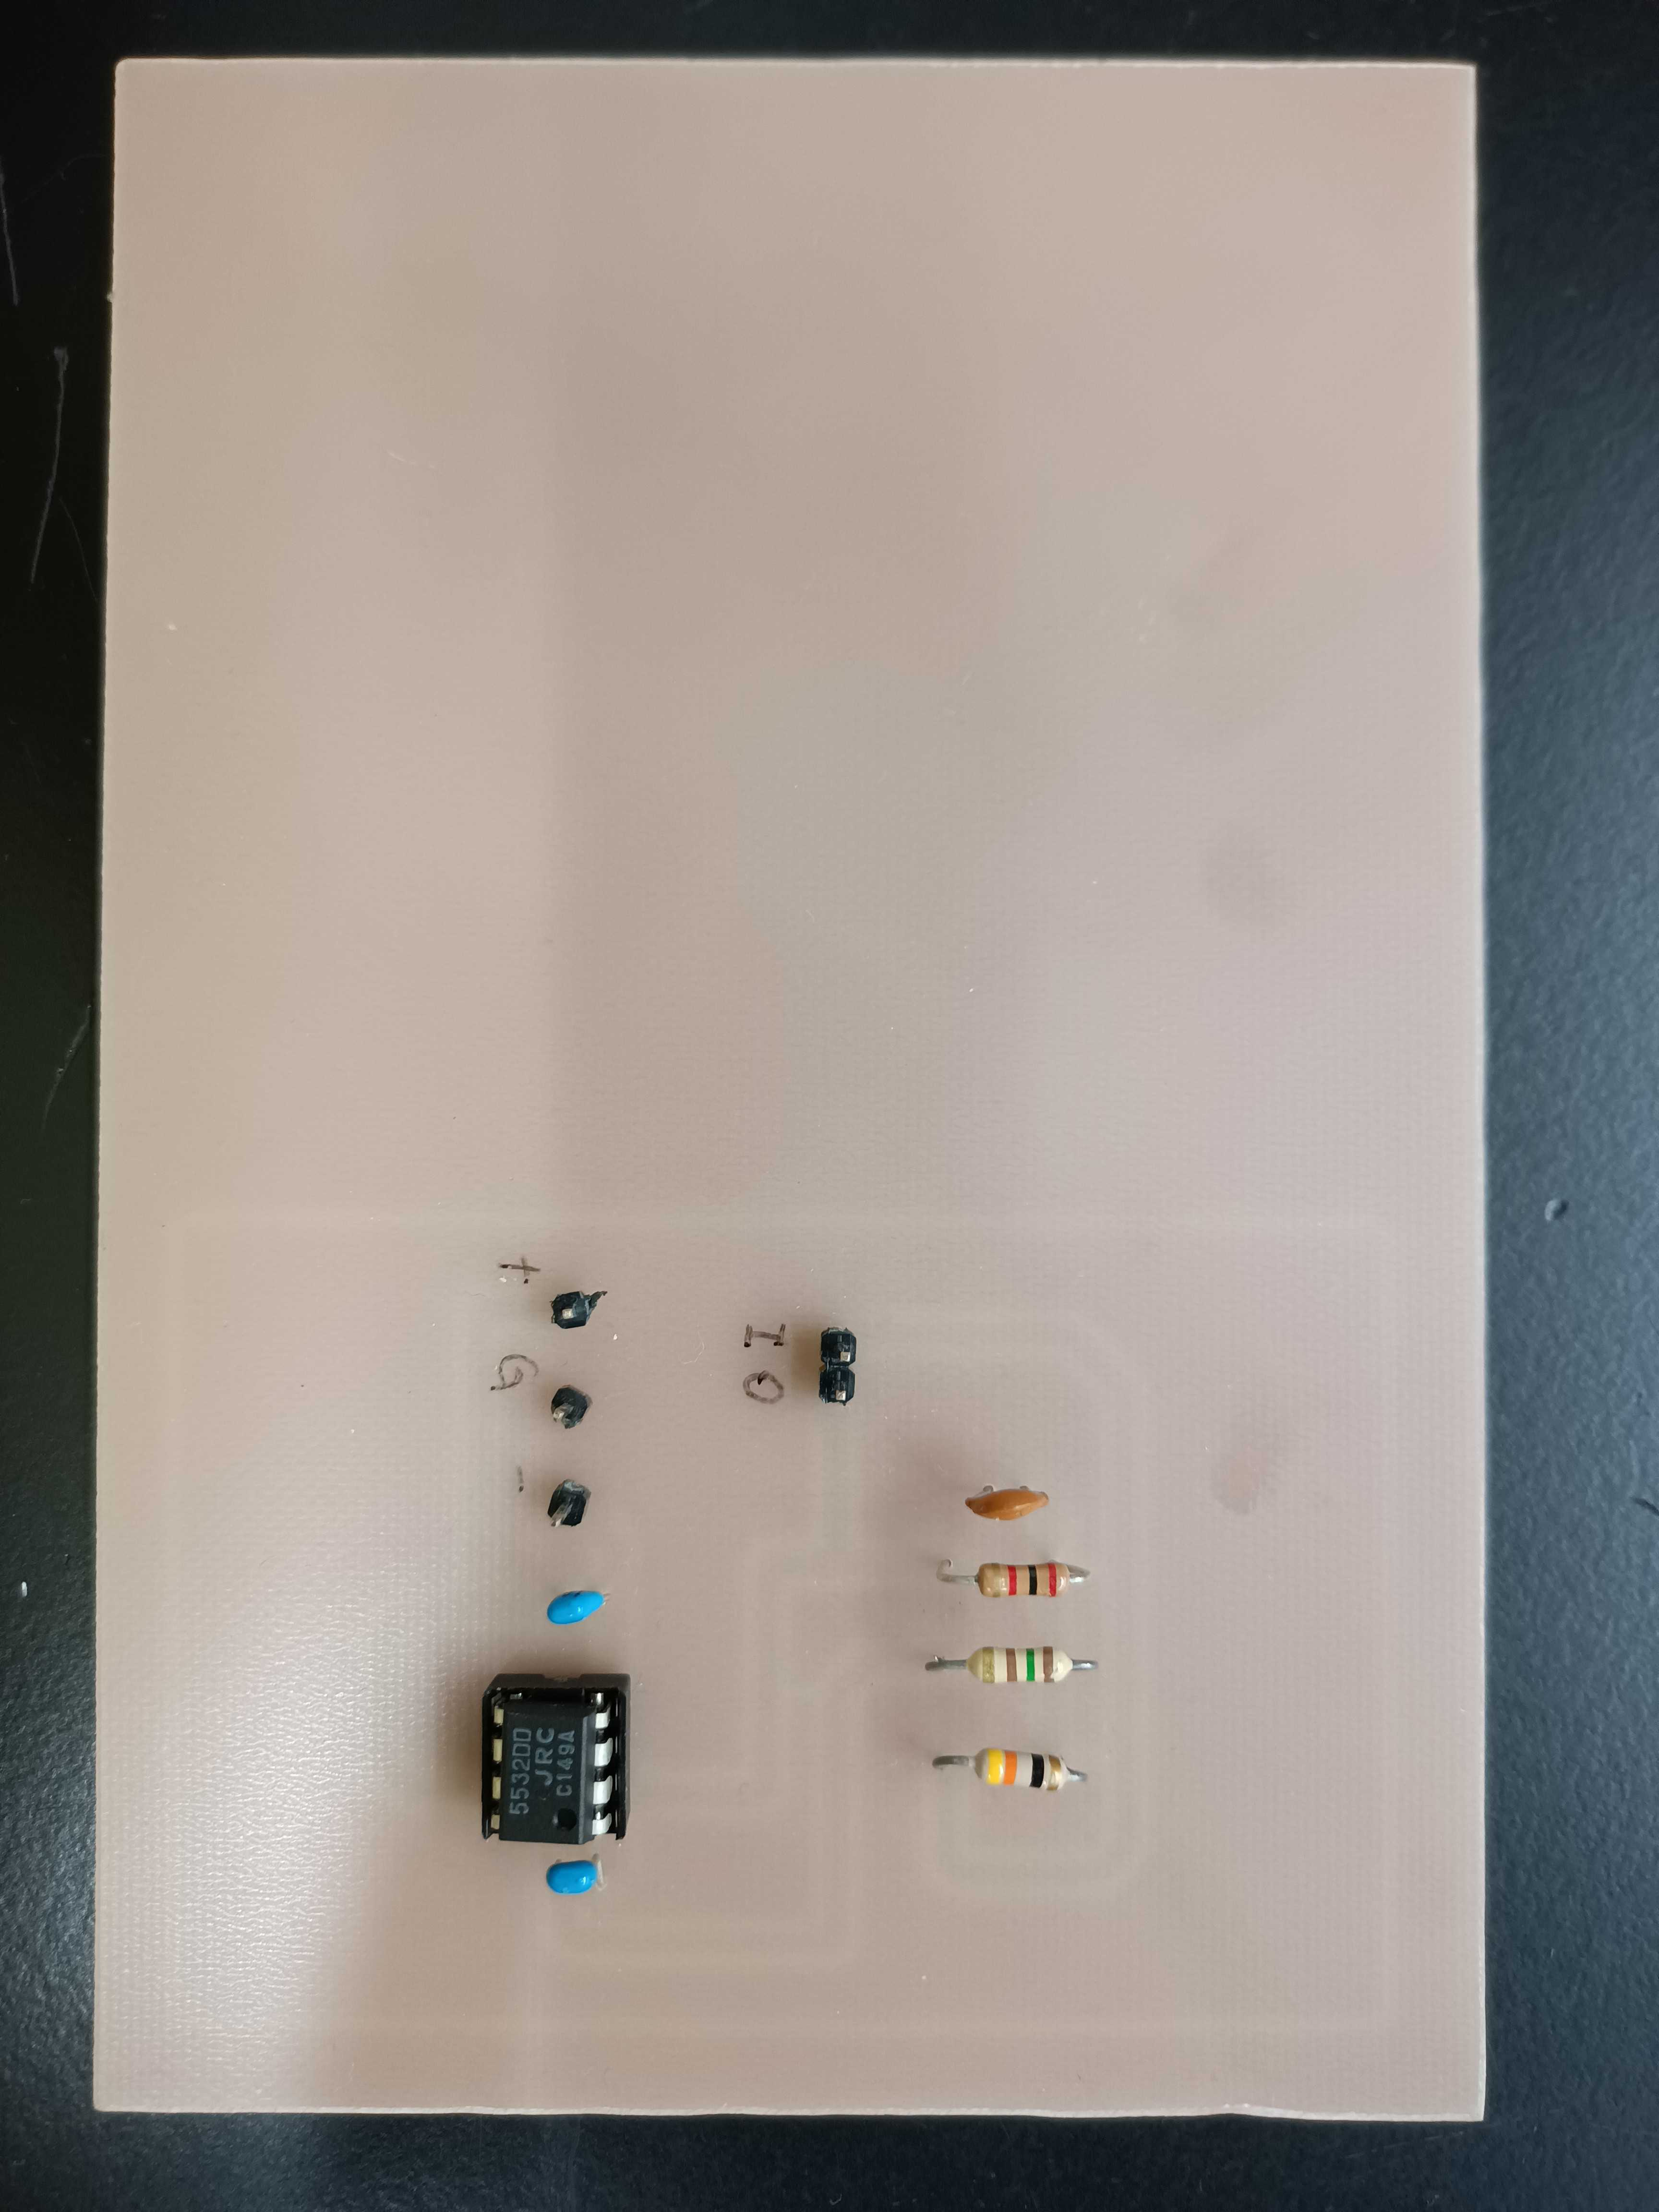
\includegraphics[width=7cm]{use/1.jpg}
	\caption{かご}
	\label{fig:kago}
\end{figure}

様々な巻数で電波の受信感度を測定できたらいいのではないかと思い、かごにドリルで穴を開けてそこから導線を通してみようと考えた。
しかし、そう思った時点では、すでにかなりの巻数を巻いてしまっていたので、穴を開けるために巻いてしまった部分をやり直したり、かごについていた出っ張りの部分が邪魔であったりして、穴を開けるのが非常に困難であったり、穴を想定よりかなりズレたところに開けてしまったりして、かごでやったのは絶対に失敗したと感じた。
また、「それだとコイルが斜めっているからちゃんとアンテナとして機能しないんじゃないの?」と言われ、かごに巻き付けるのを断念した。
これは、かごが斜めっていると、想定していたインダクタンス値からかなりズレてしまうと思ったからである。


\subsubsection{エナメル線}

最初に、0.32mmの導線でアンテナを巻き付ける際に、秋葉原で売っていた20mのエナメル線を用いた。
袋を開けてから、何も考えずにすぐに巻き付けようとしてしまった。そのせいで導線がどんどんと絡まってしまった。
その時、竹中が開封したときは、きれいな導線だったから引っ張ればもとに戻ると勘違いしてしまい、他の二人がそれは良くないと言っていたが、気づいたときには、元には戻せないほど絡まってしまった。

\subsection{フィルタ回路の作成}

角張の高い音と低い音をカットするローパスフィルターとハイパスフィルターの回路を参考にして、ノイズや発振をカットしてくれるアクティブフィルタの作成をしてもらった。
しかし、フェムトファラッド単位のコンデンサが必要になり、作業が難航した。
何とか頑張って\wfig{filter}のような回路を作成してもらった。
しかし、電源を用いて回路を作動させたところ、電源が短絡してしまっていた。
結局のところ原因がわからず、フィルタ回路を作成することはできなかった。

\begin{figure}[H]
	\centering
	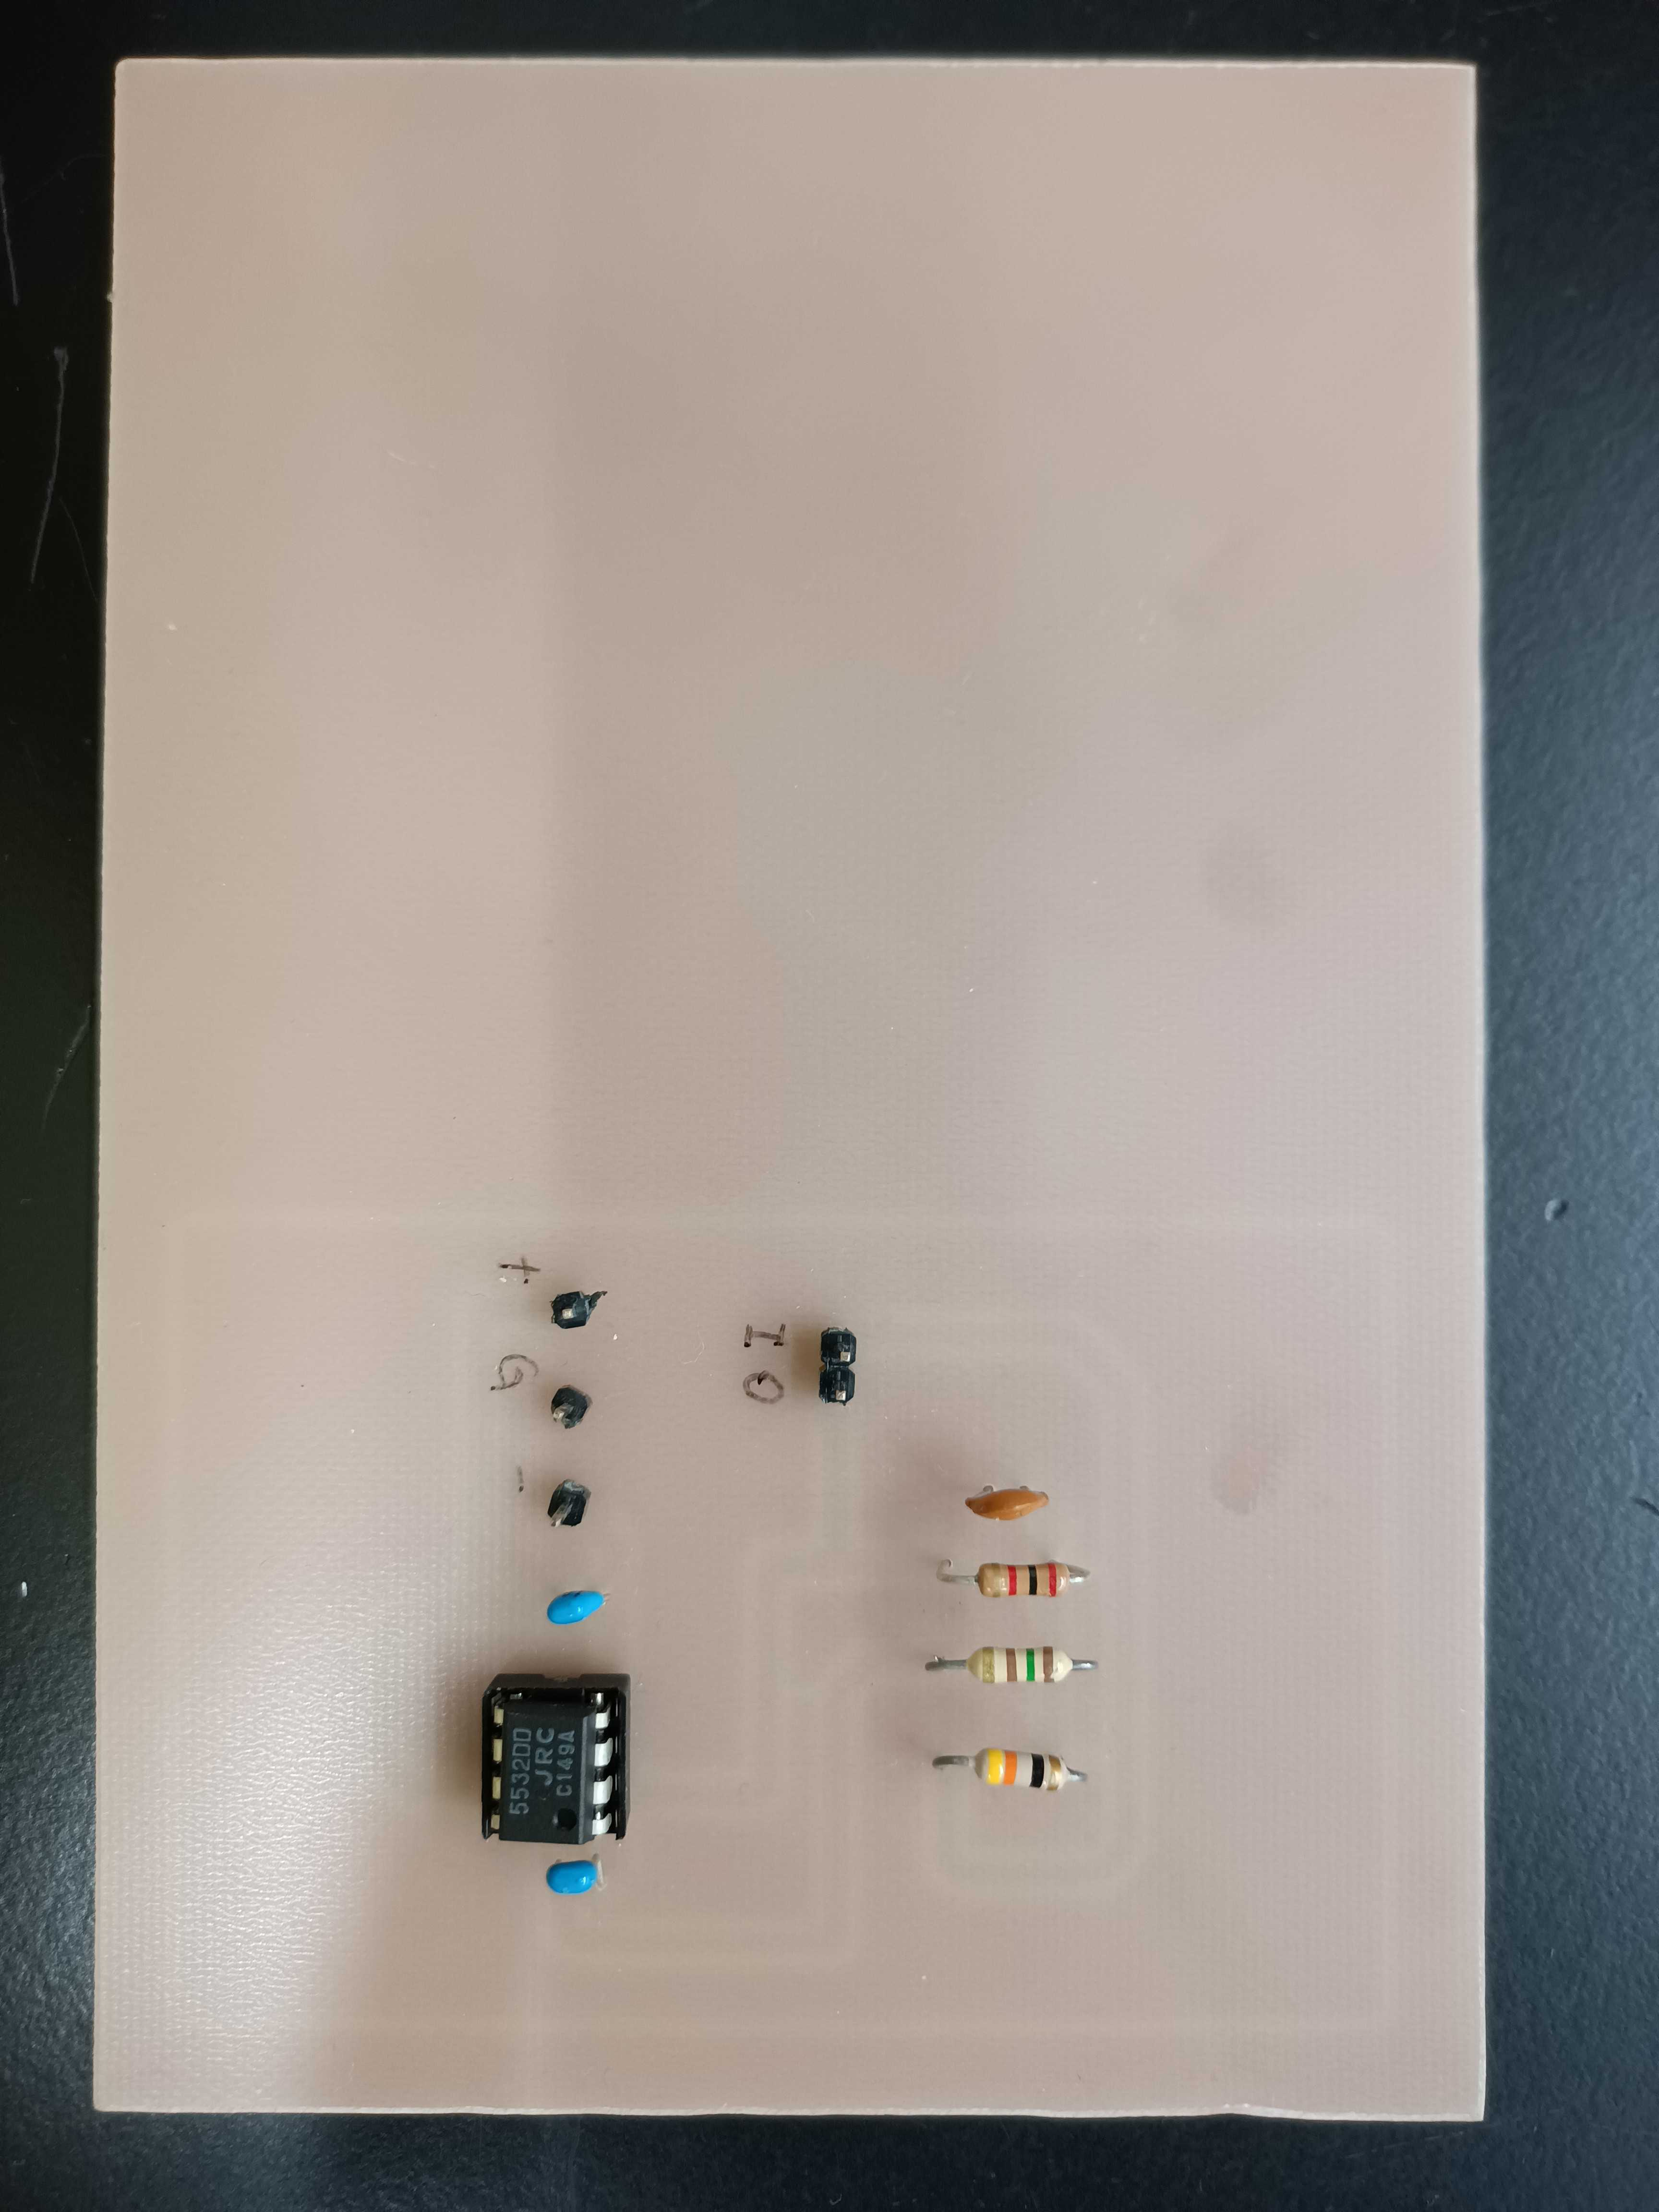
\includegraphics[width=7cm]{use/1.jpg}
	\caption{フィルタ回路}
	\label{fig:filter}
\end{figure}

\subsection{増幅回路の作成}

\begin{figure}[H]
	\begin{minipage}[b]{0.5\linewidth}
		\centering
		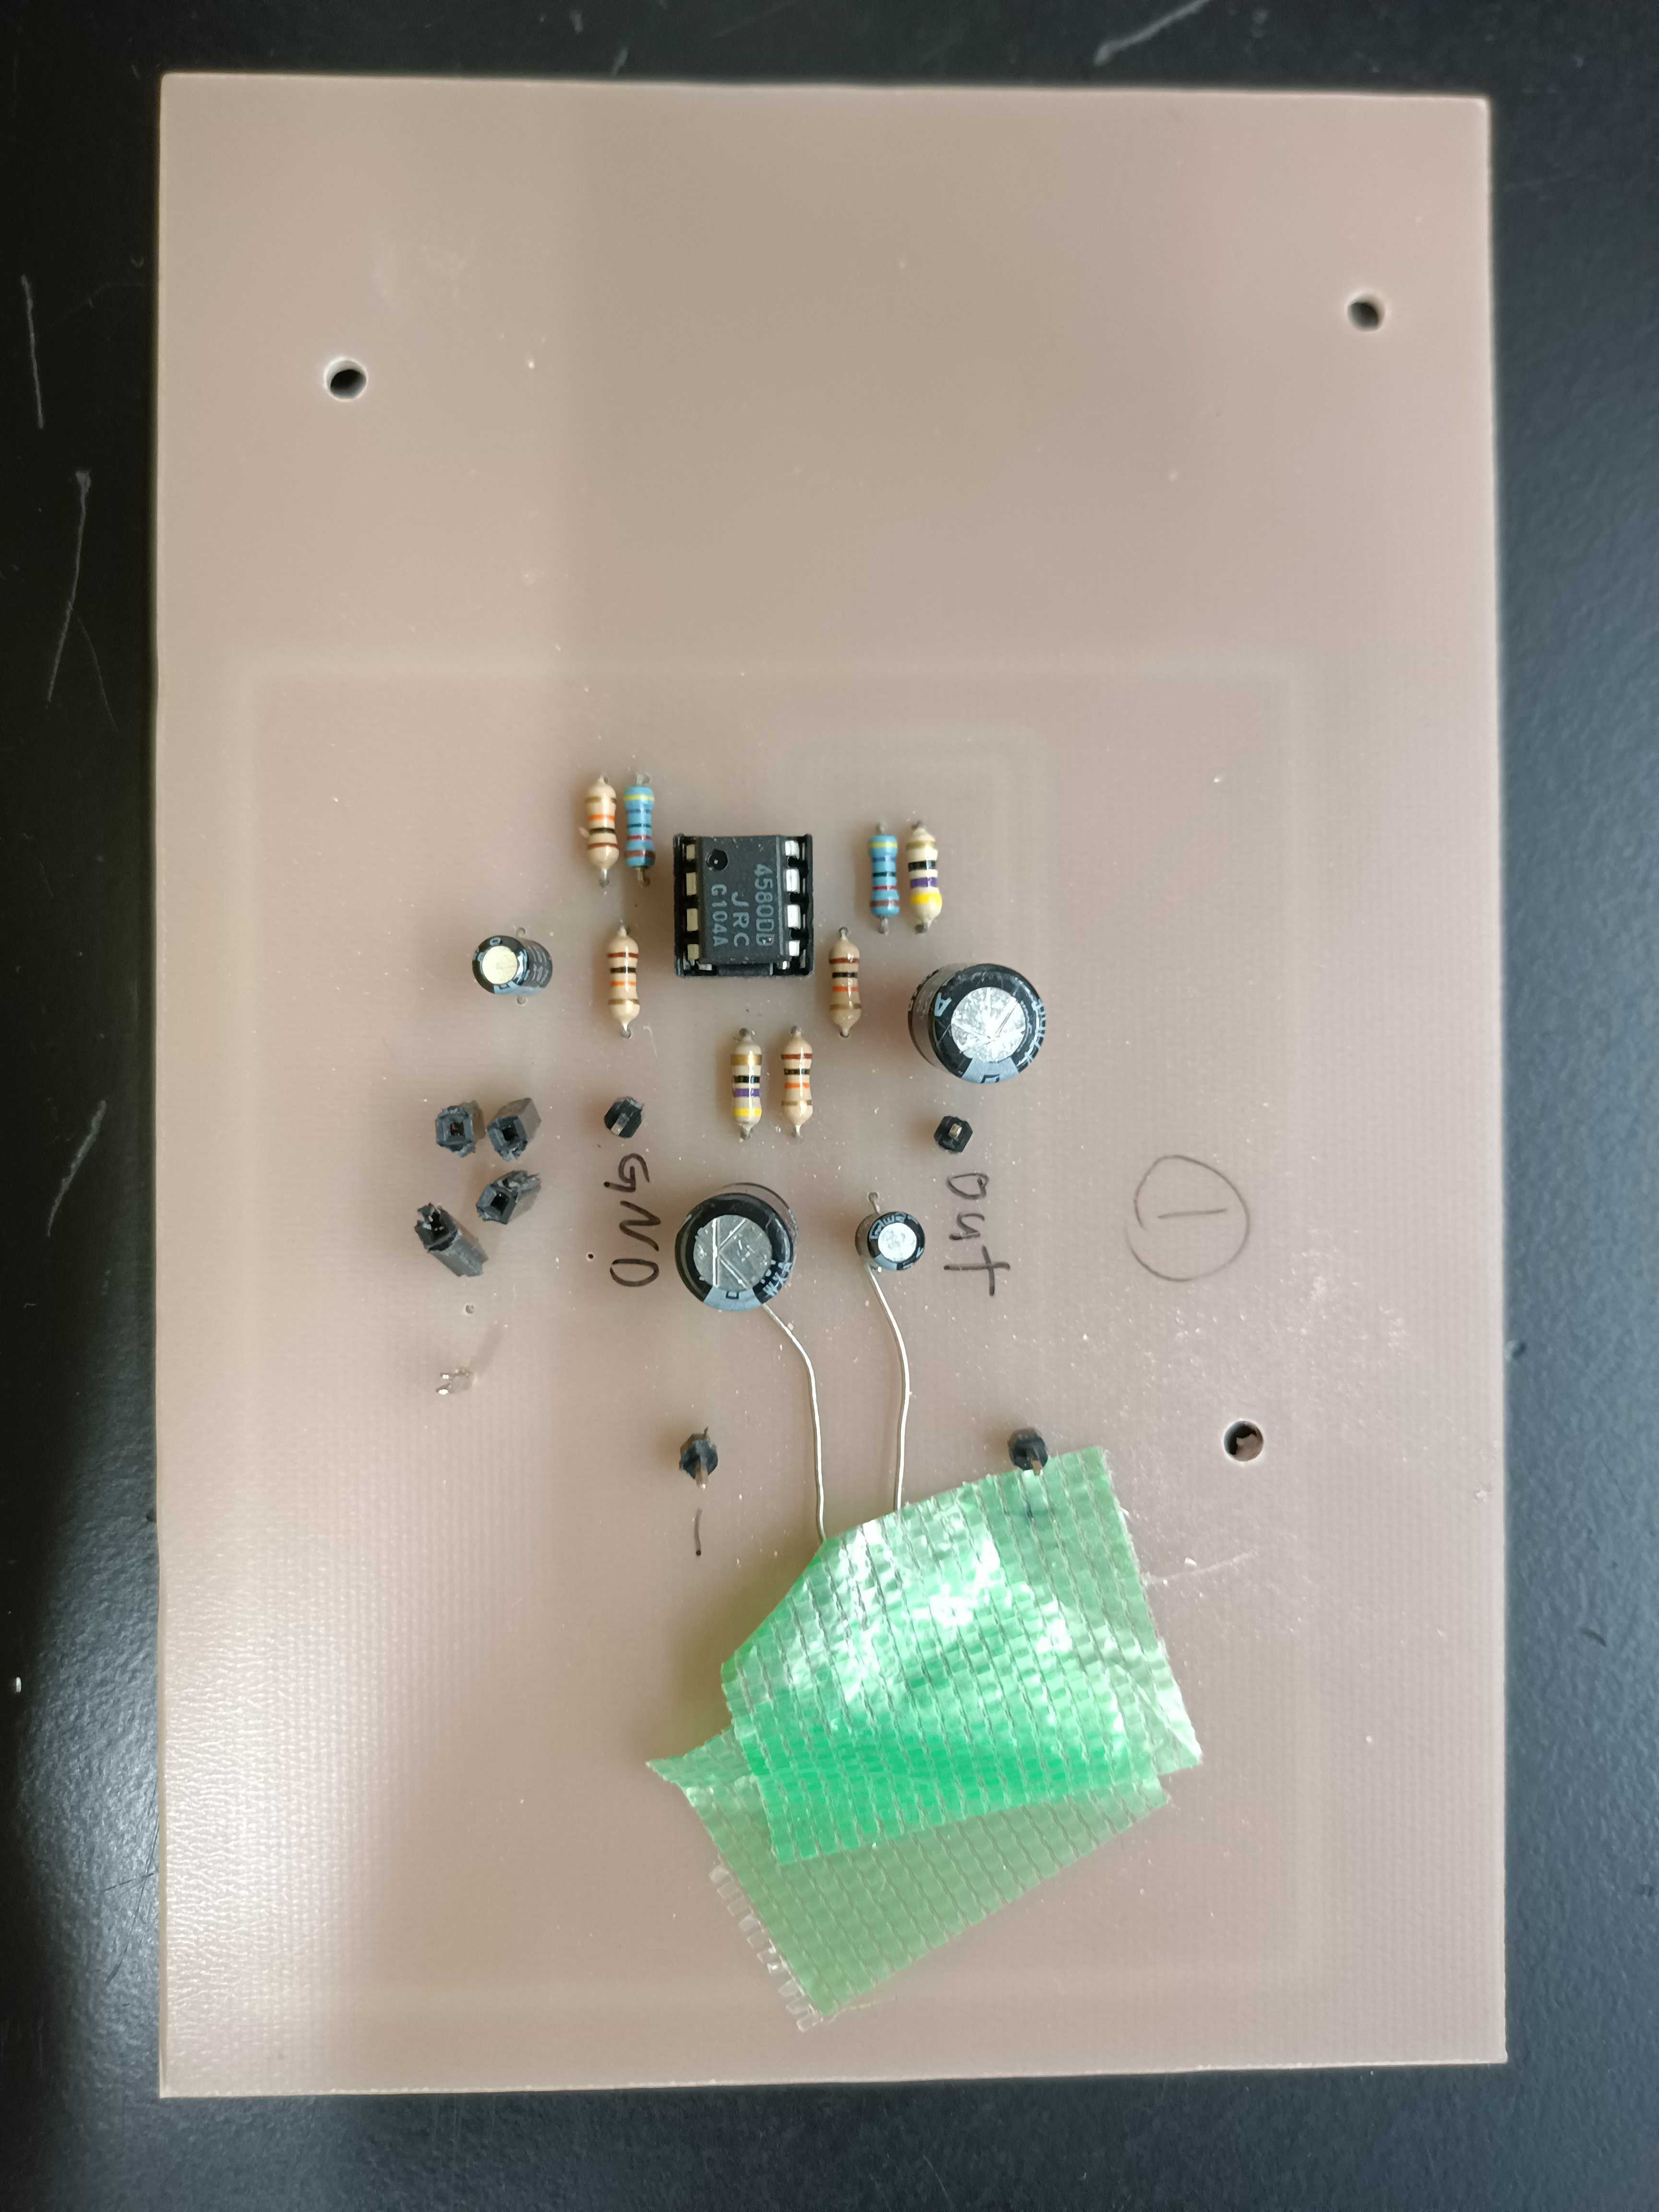
\includegraphics[width=8cm]{use/2.jpg}
		\caption{アンプ一台目}
		\label{fig:s_2}
	\end{minipage}
	\begin{minipage}[b]{0.5\linewidth}
		\centering
		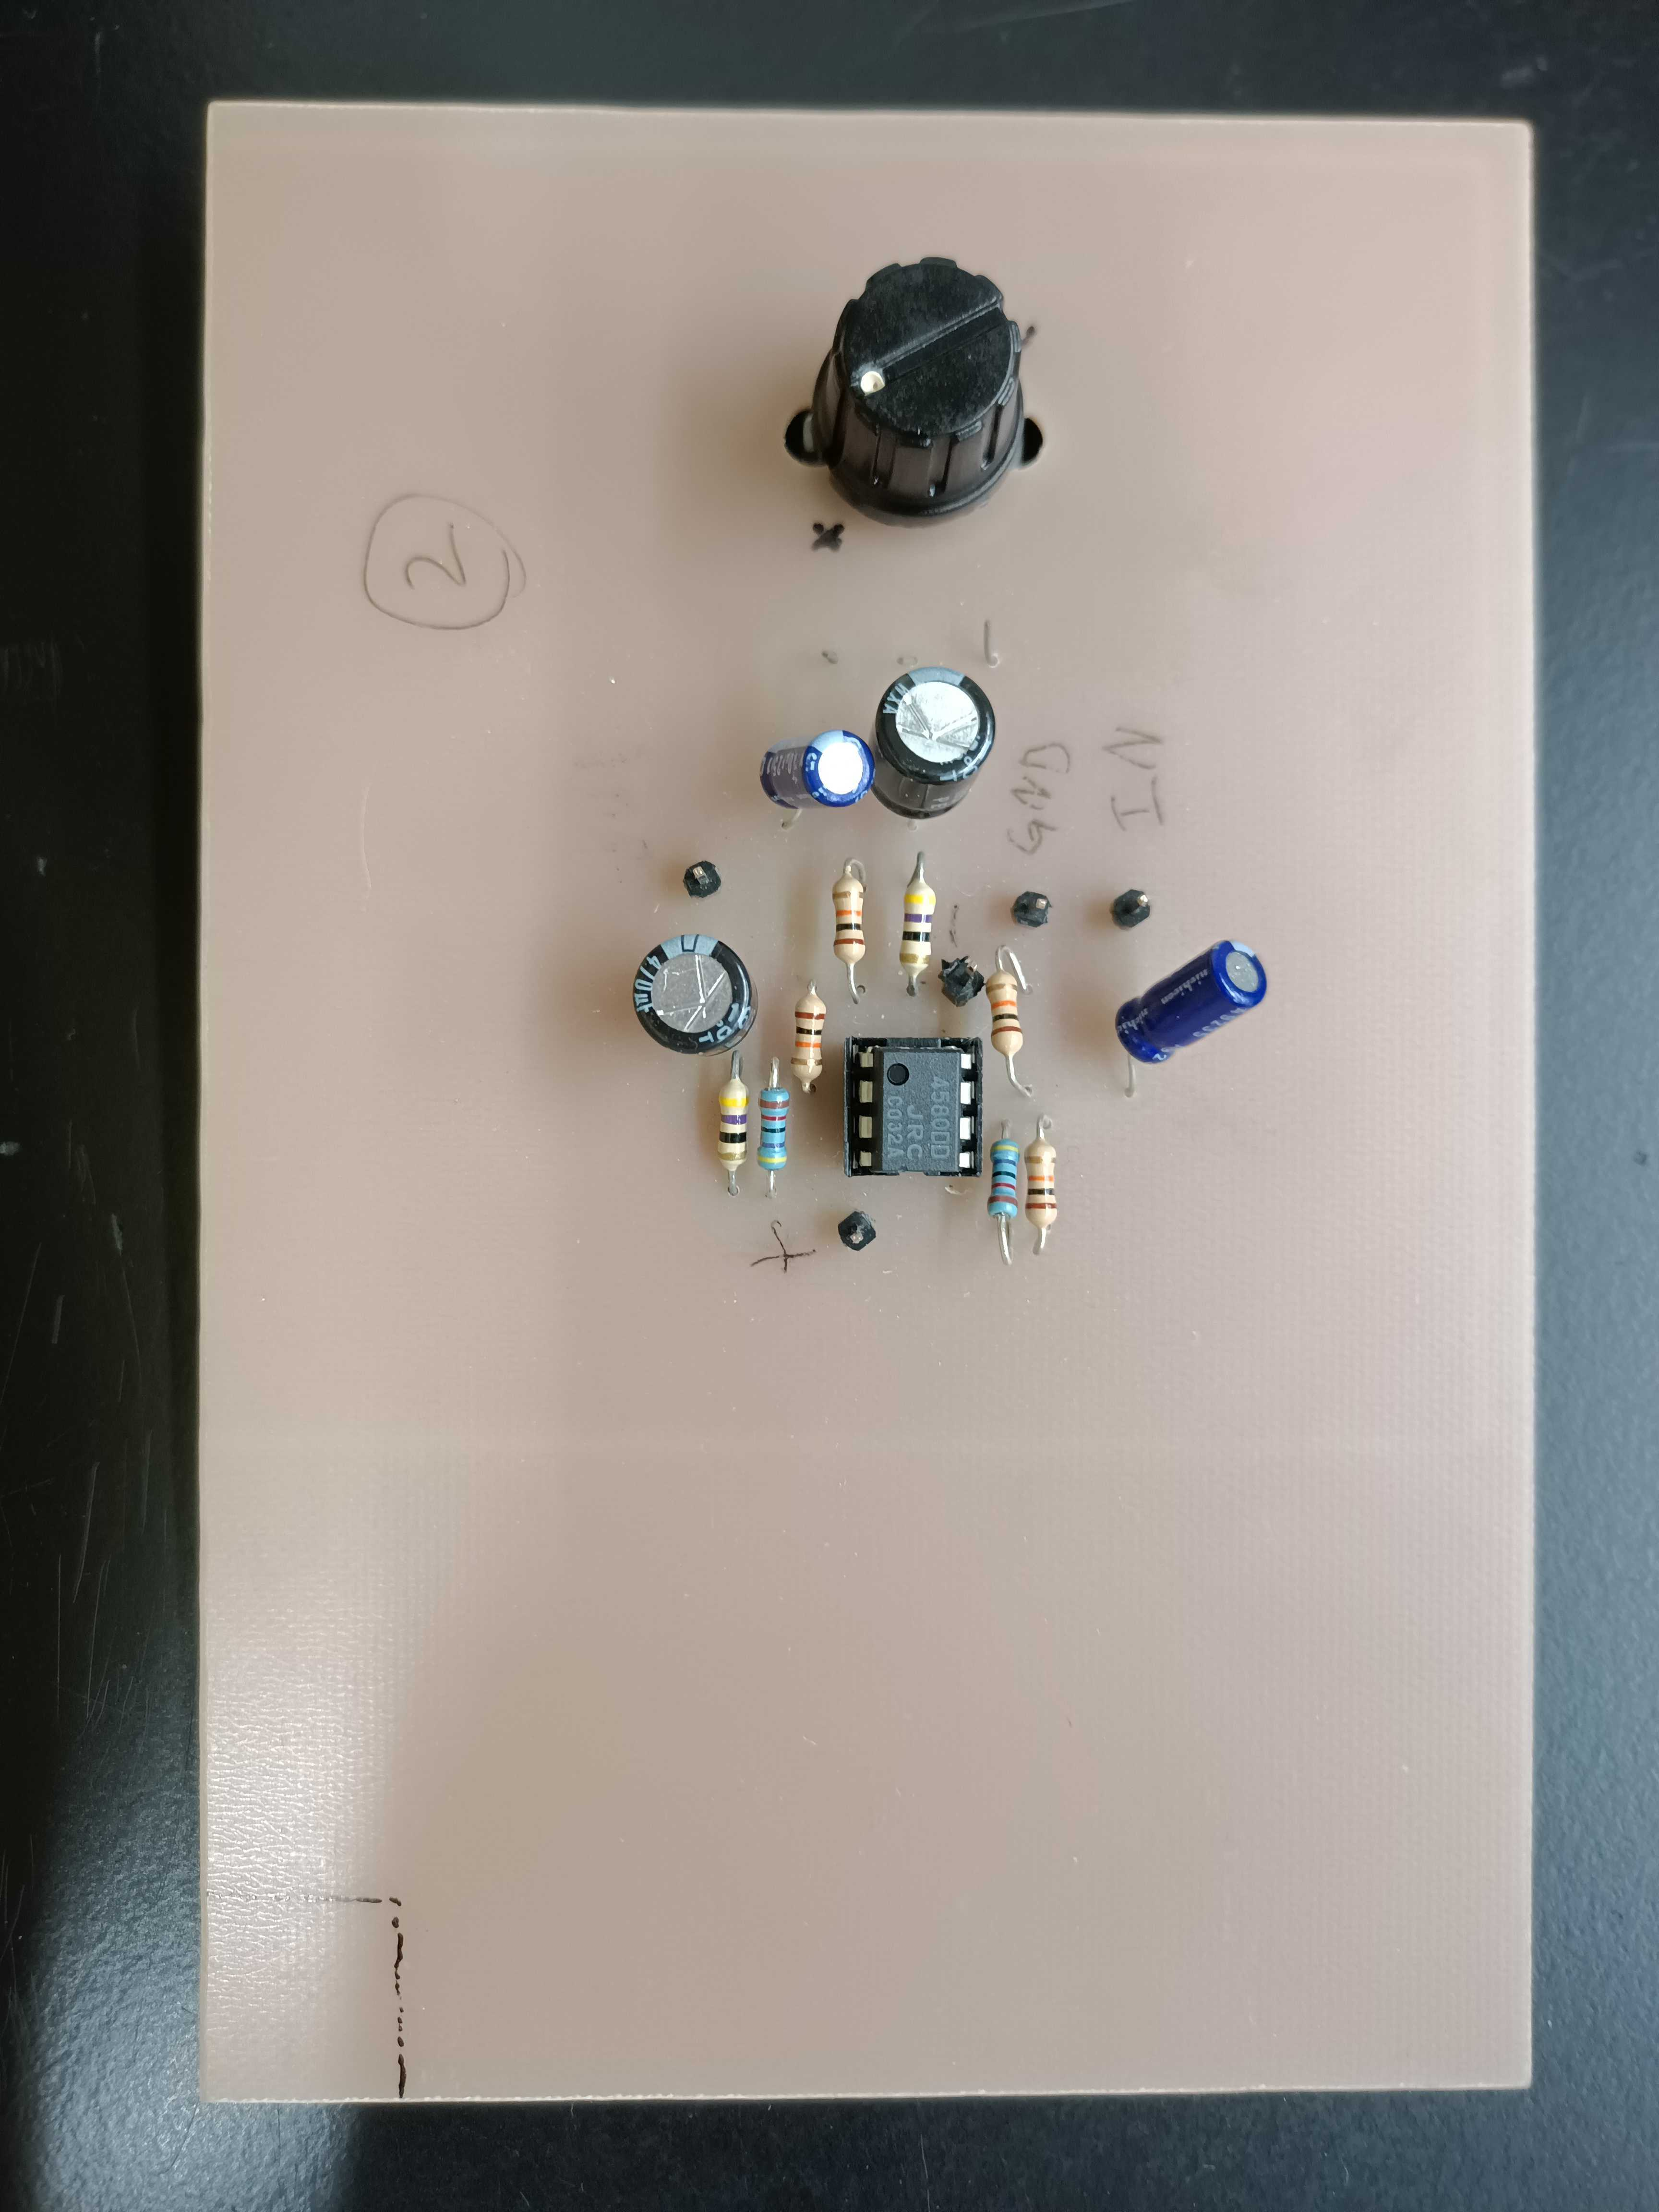
\includegraphics[width=8cm]{use/3.jpg}
		\caption{アンプ二台目}
		\label{fig:s_3}
	\end{minipage}
\end{figure}

\begin{figure}[H]
	\begin{minipage}[b]{0.5\linewidth}
		\centering
		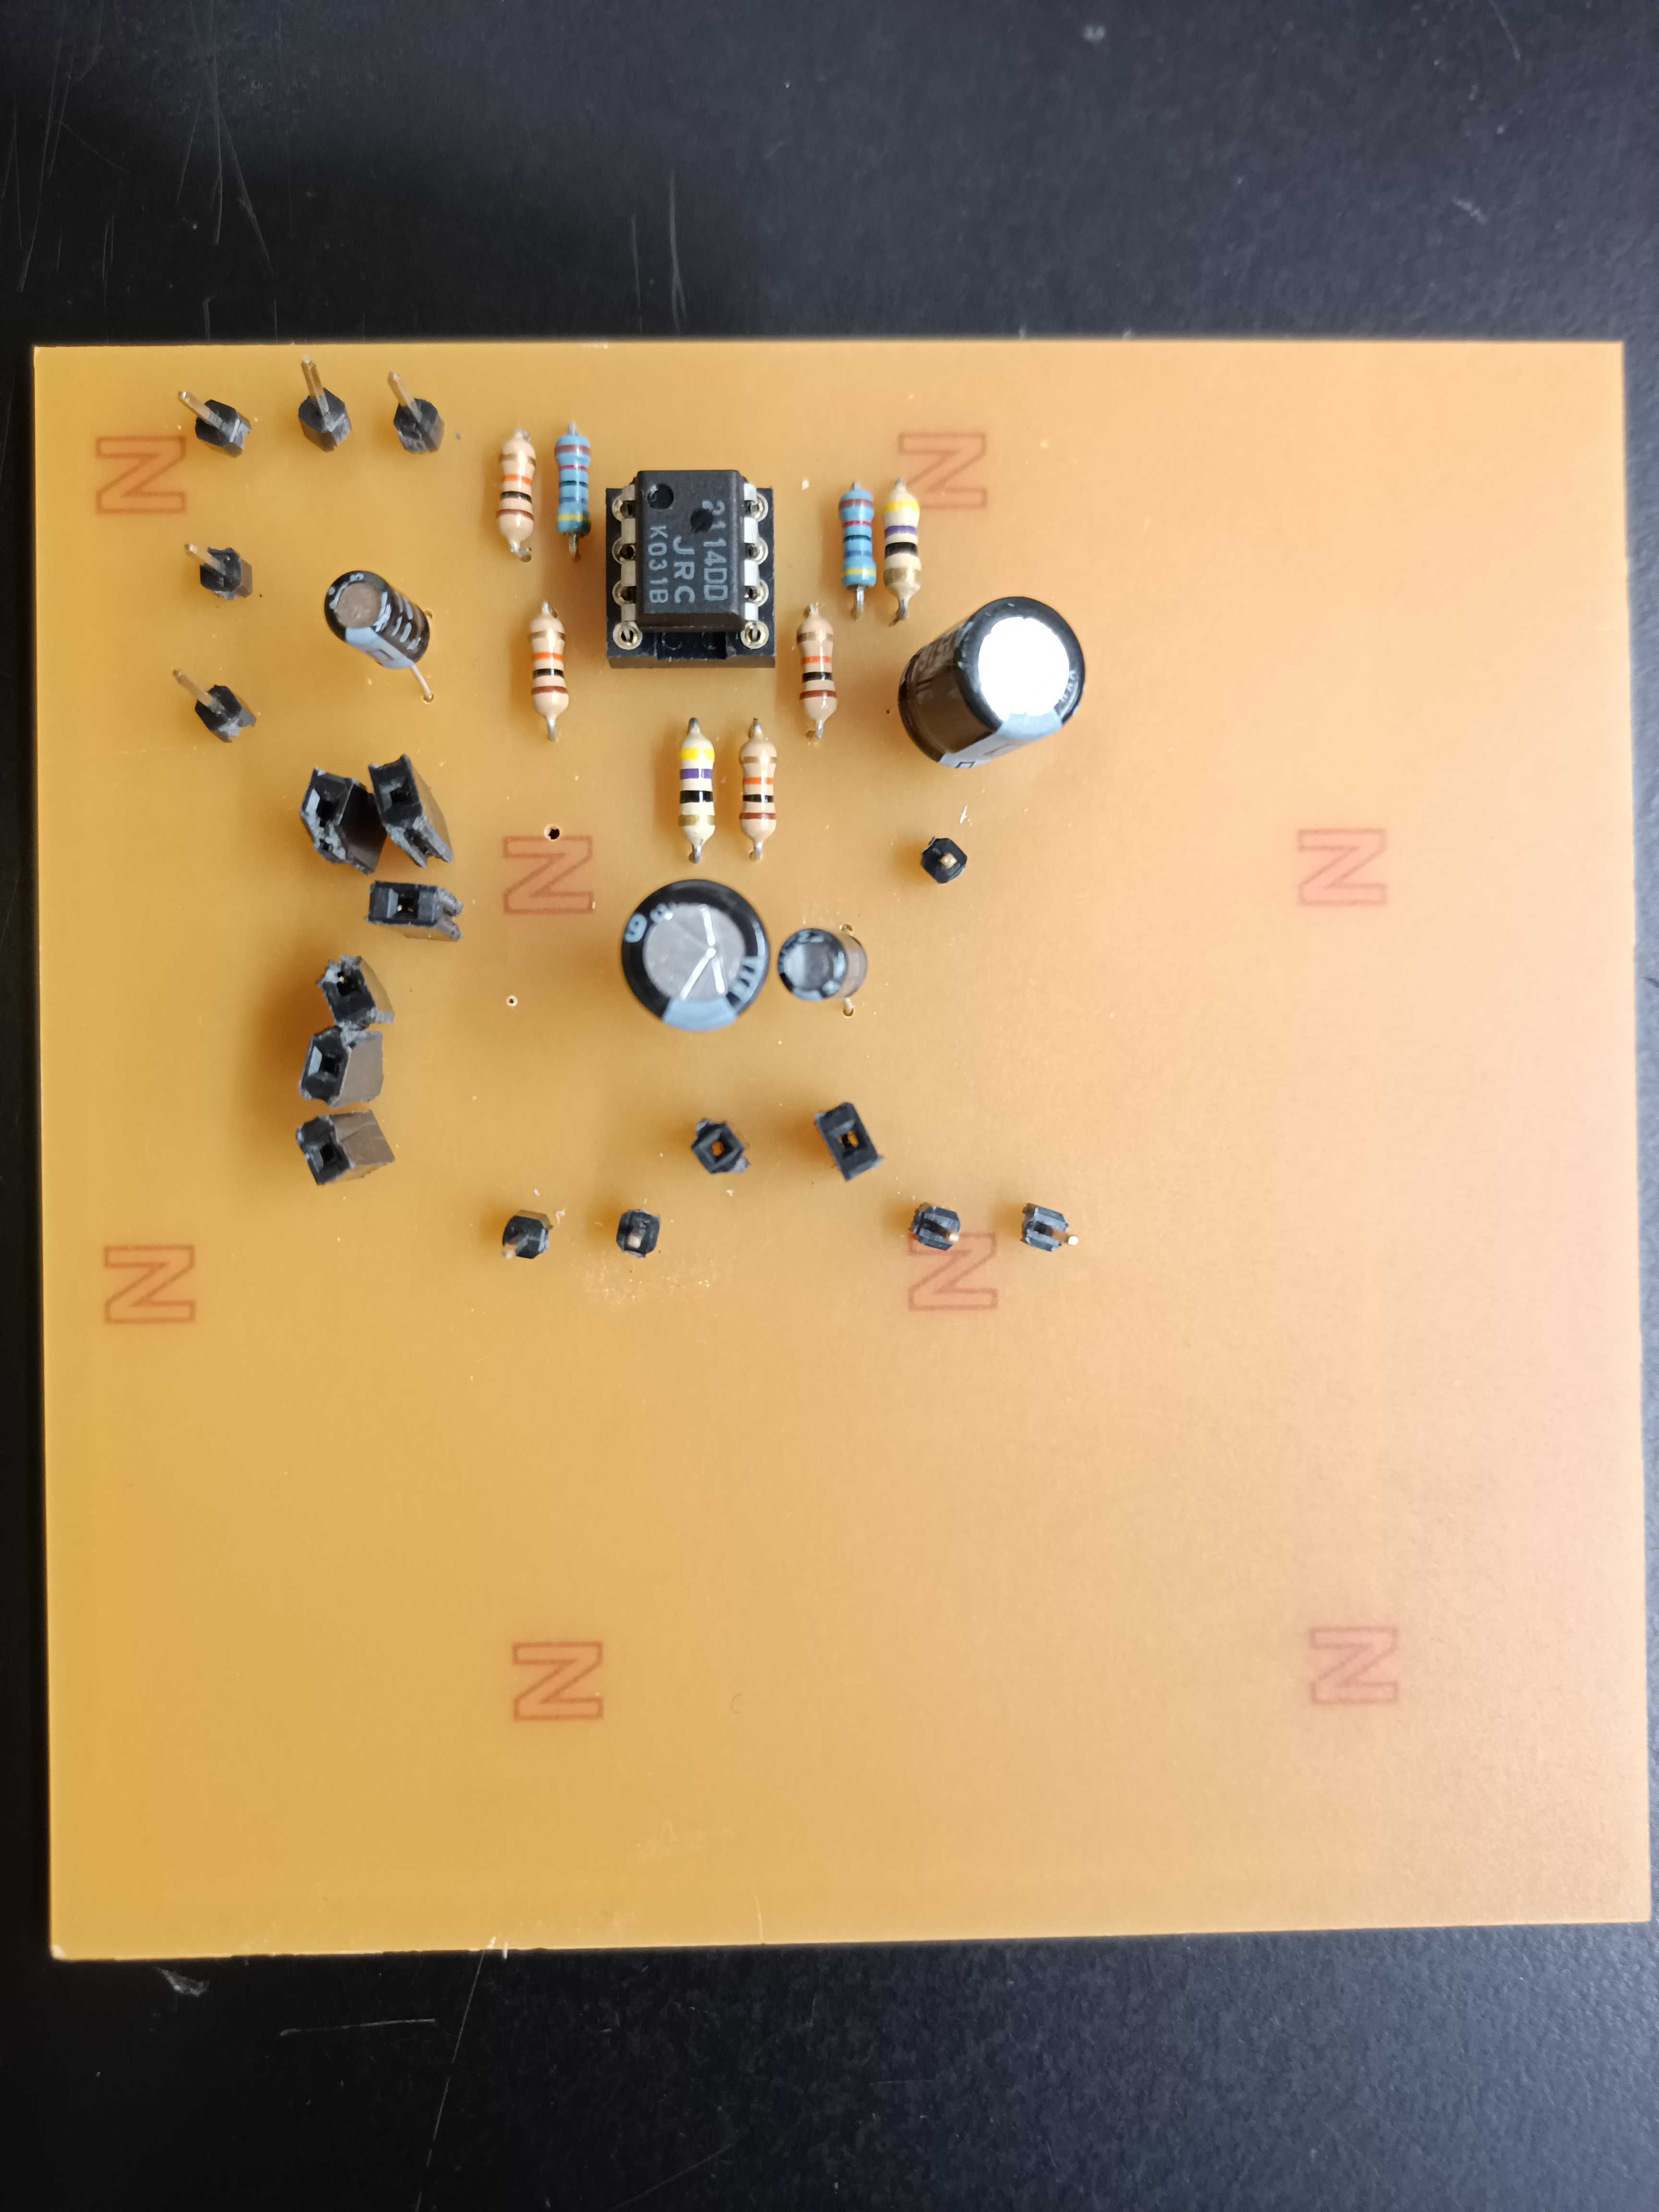
\includegraphics[width=8cm]{use/5.jpg}
		\caption{アンプ三台目}
		\label{fig:s_4}
	\end{minipage}
	\begin{minipage}[b]{0.5\linewidth}
		\centering
		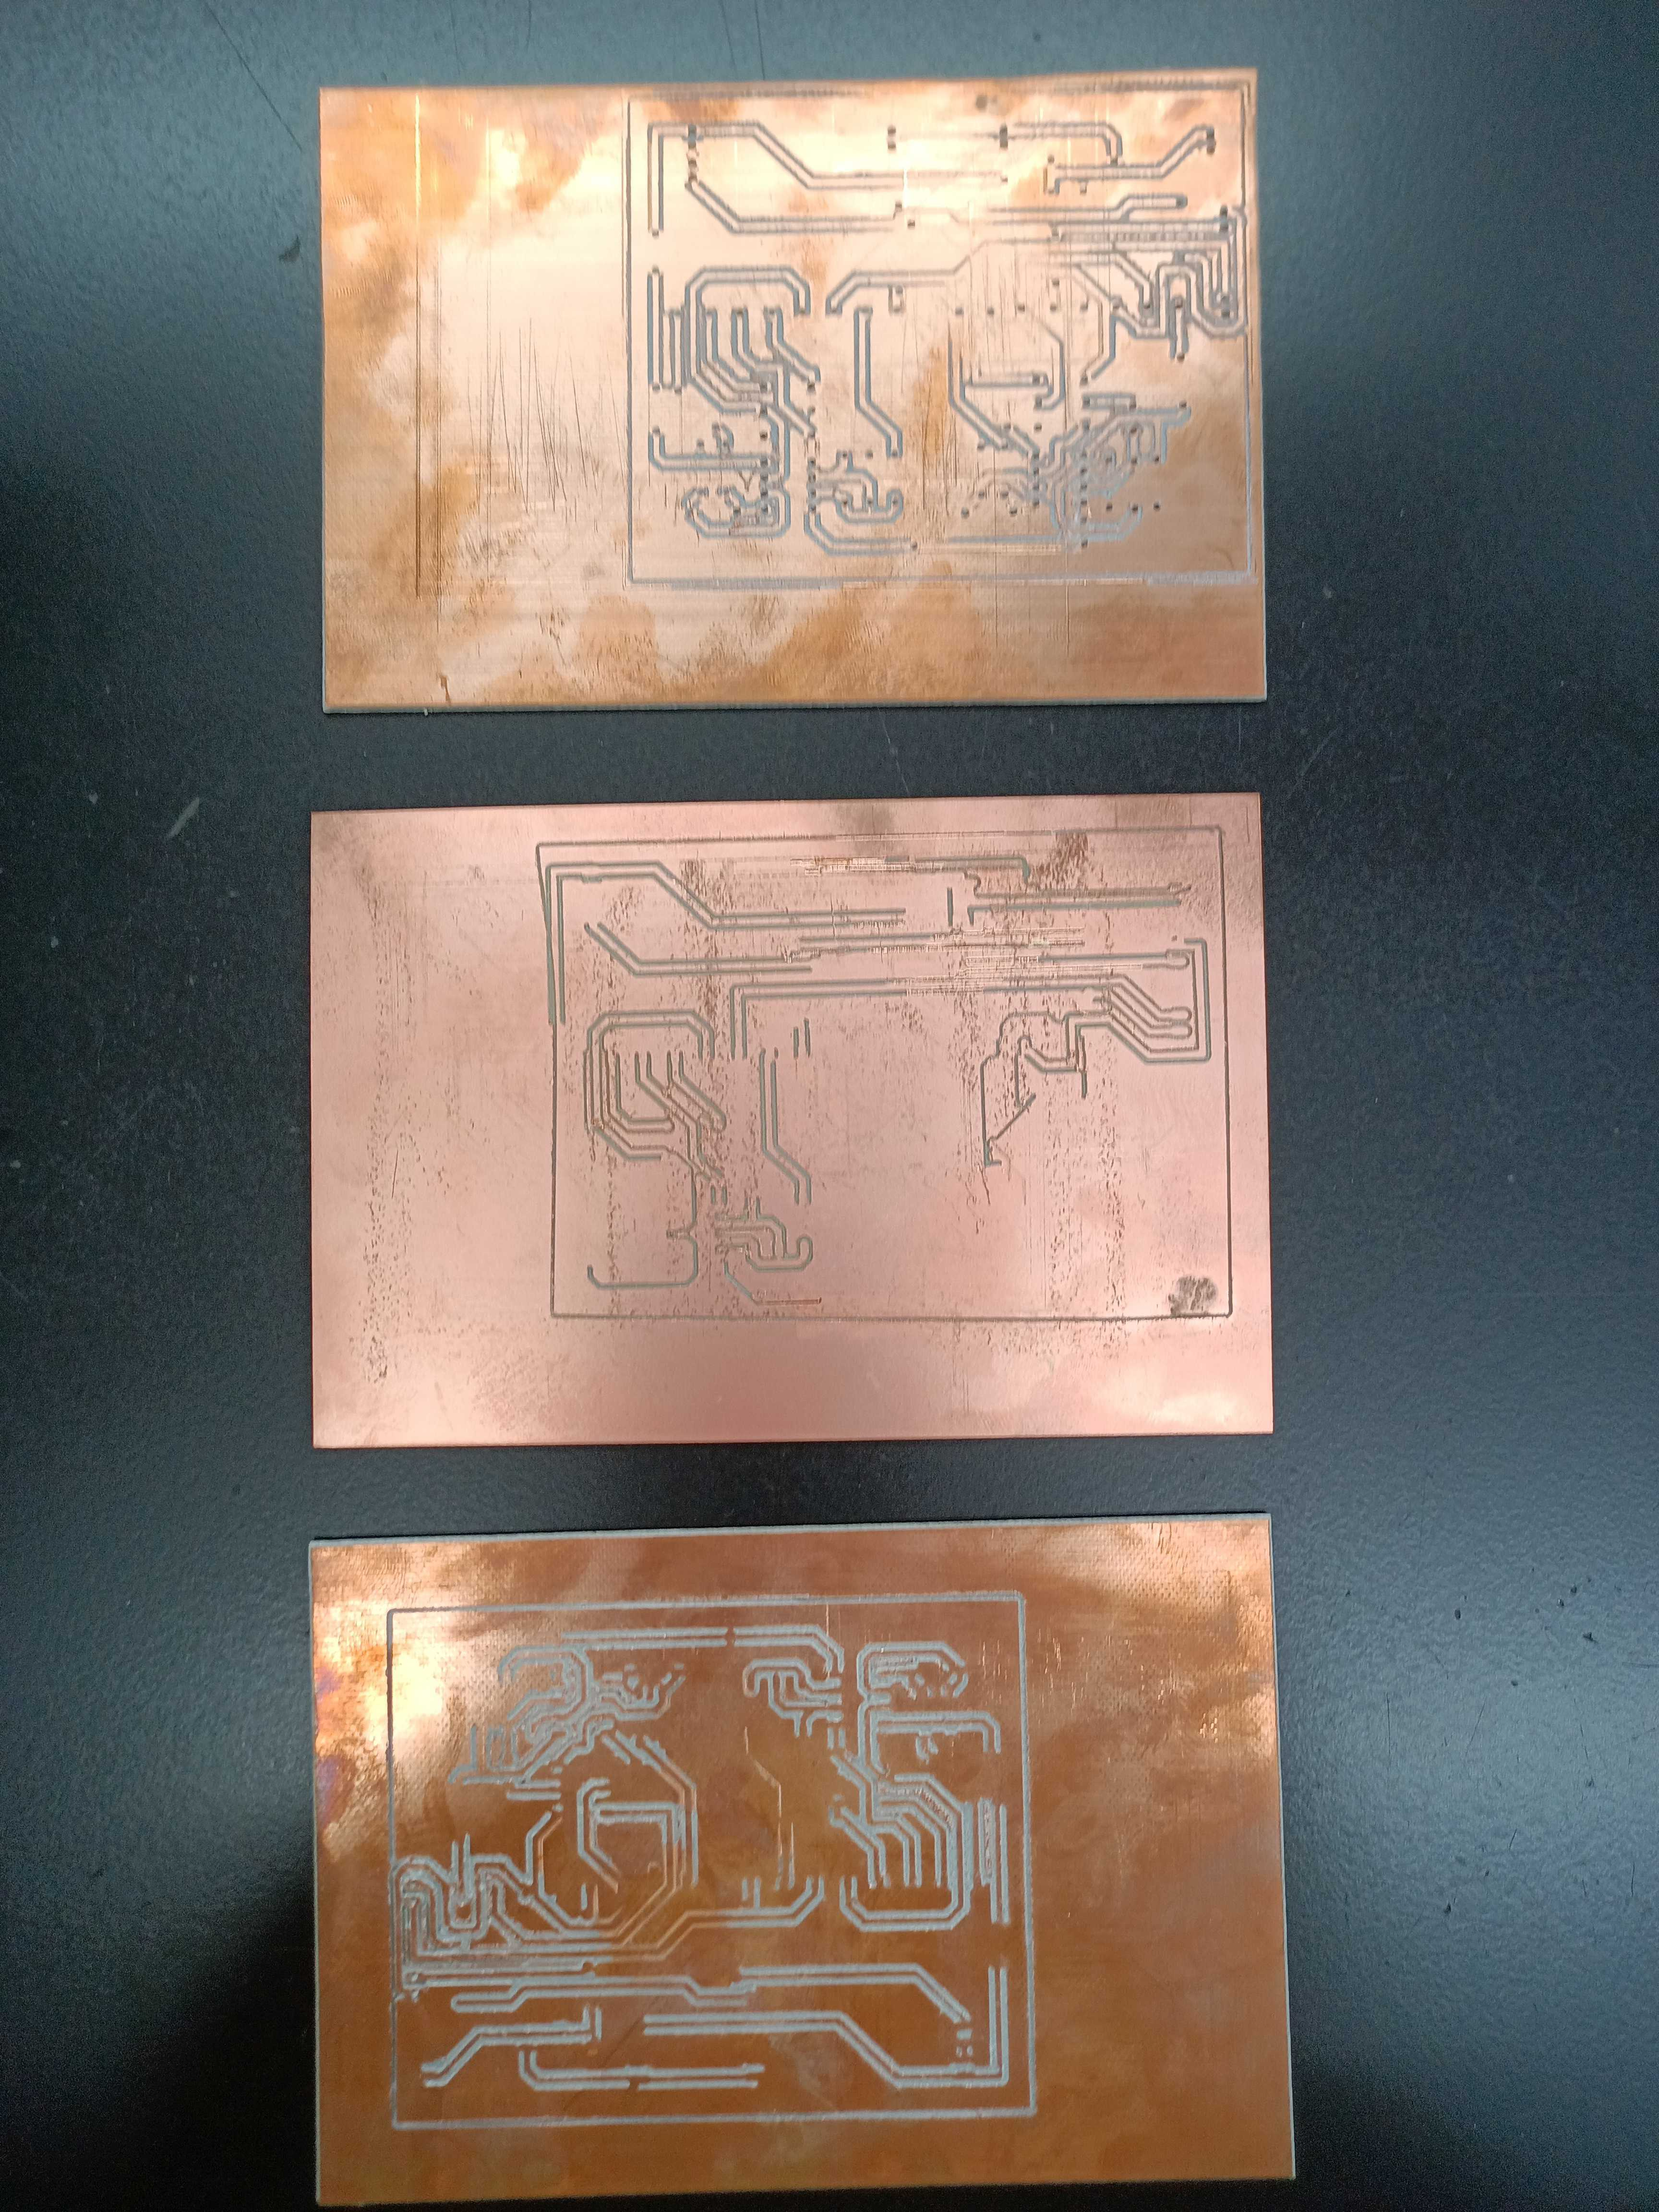
\includegraphics[width=8cm]{use/6.jpg}
		\caption{アンプ四代目になる予定だったもの}
		\label{fig:s_5}
	\end{minipage}
\end{figure}

\begin{figure}[H]
	\begin{minipage}[b]{0.5\linewidth}
		\centering
		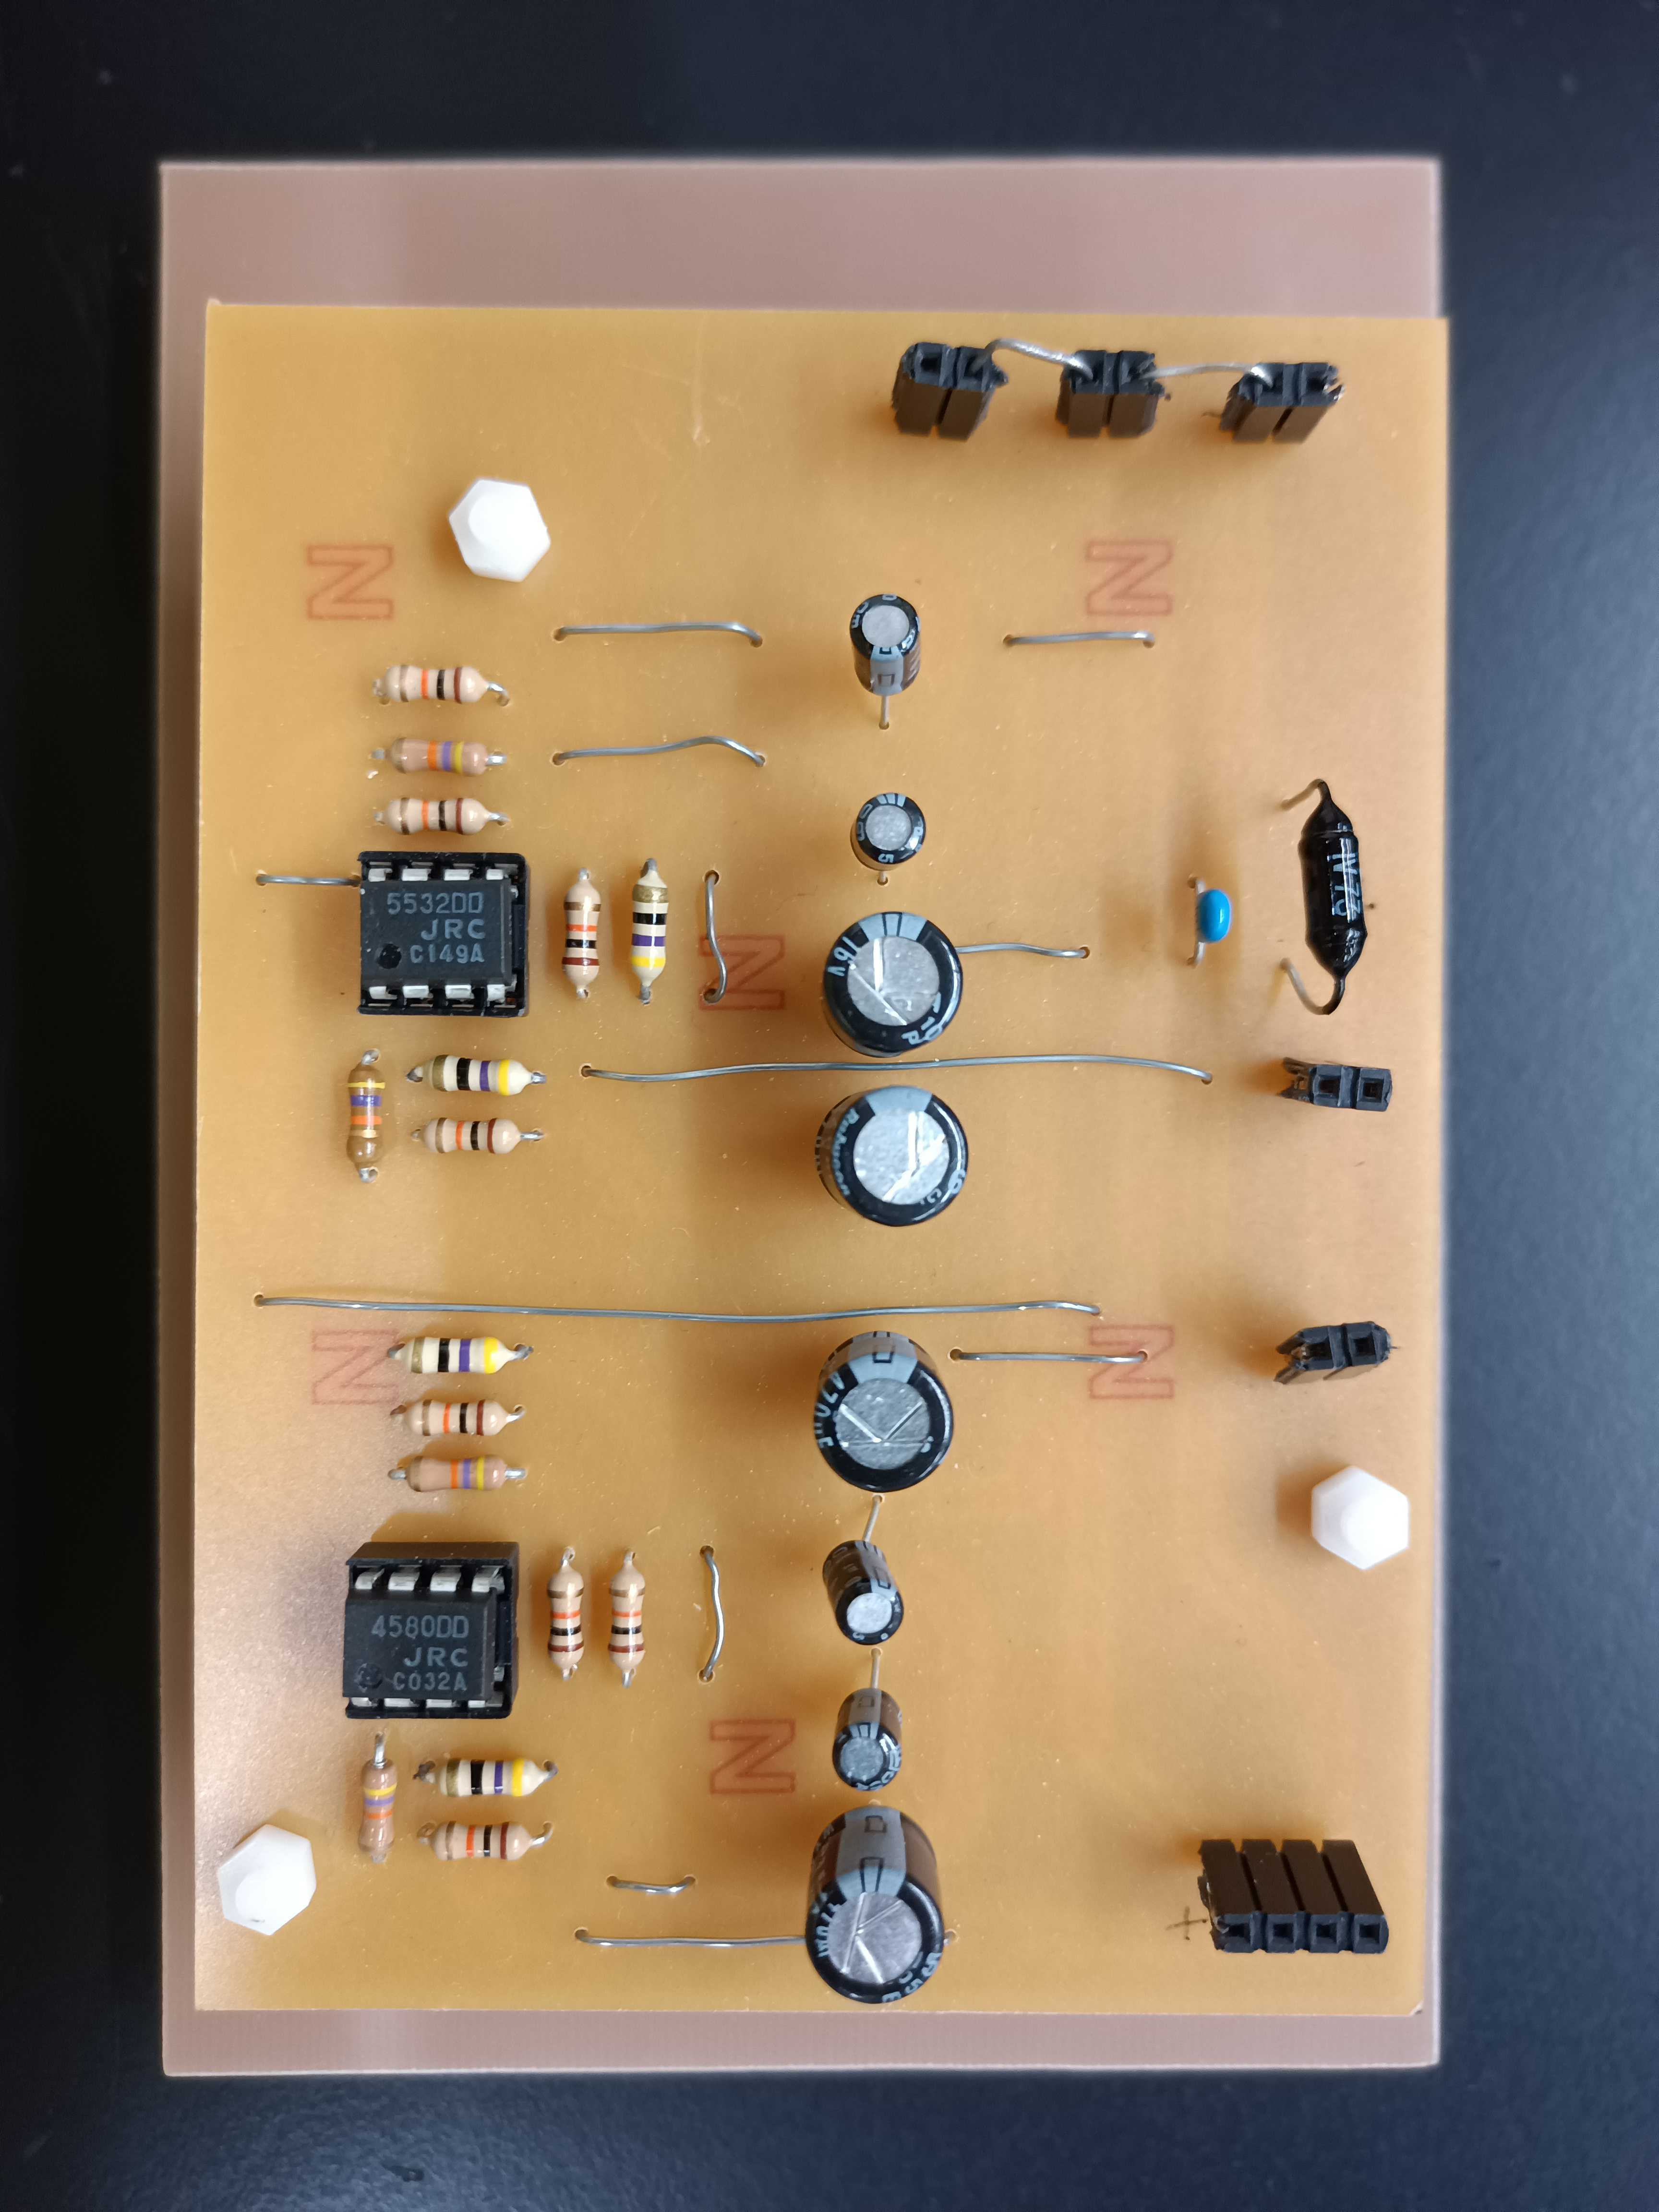
\includegraphics[width=8cm]{use/4.jpg}
		\caption{2号機アンテナの写真}
		\label{fig:s_6}
	\end{minipage}
	\begin{minipage}[b]{0.5\linewidth}
		\centering
		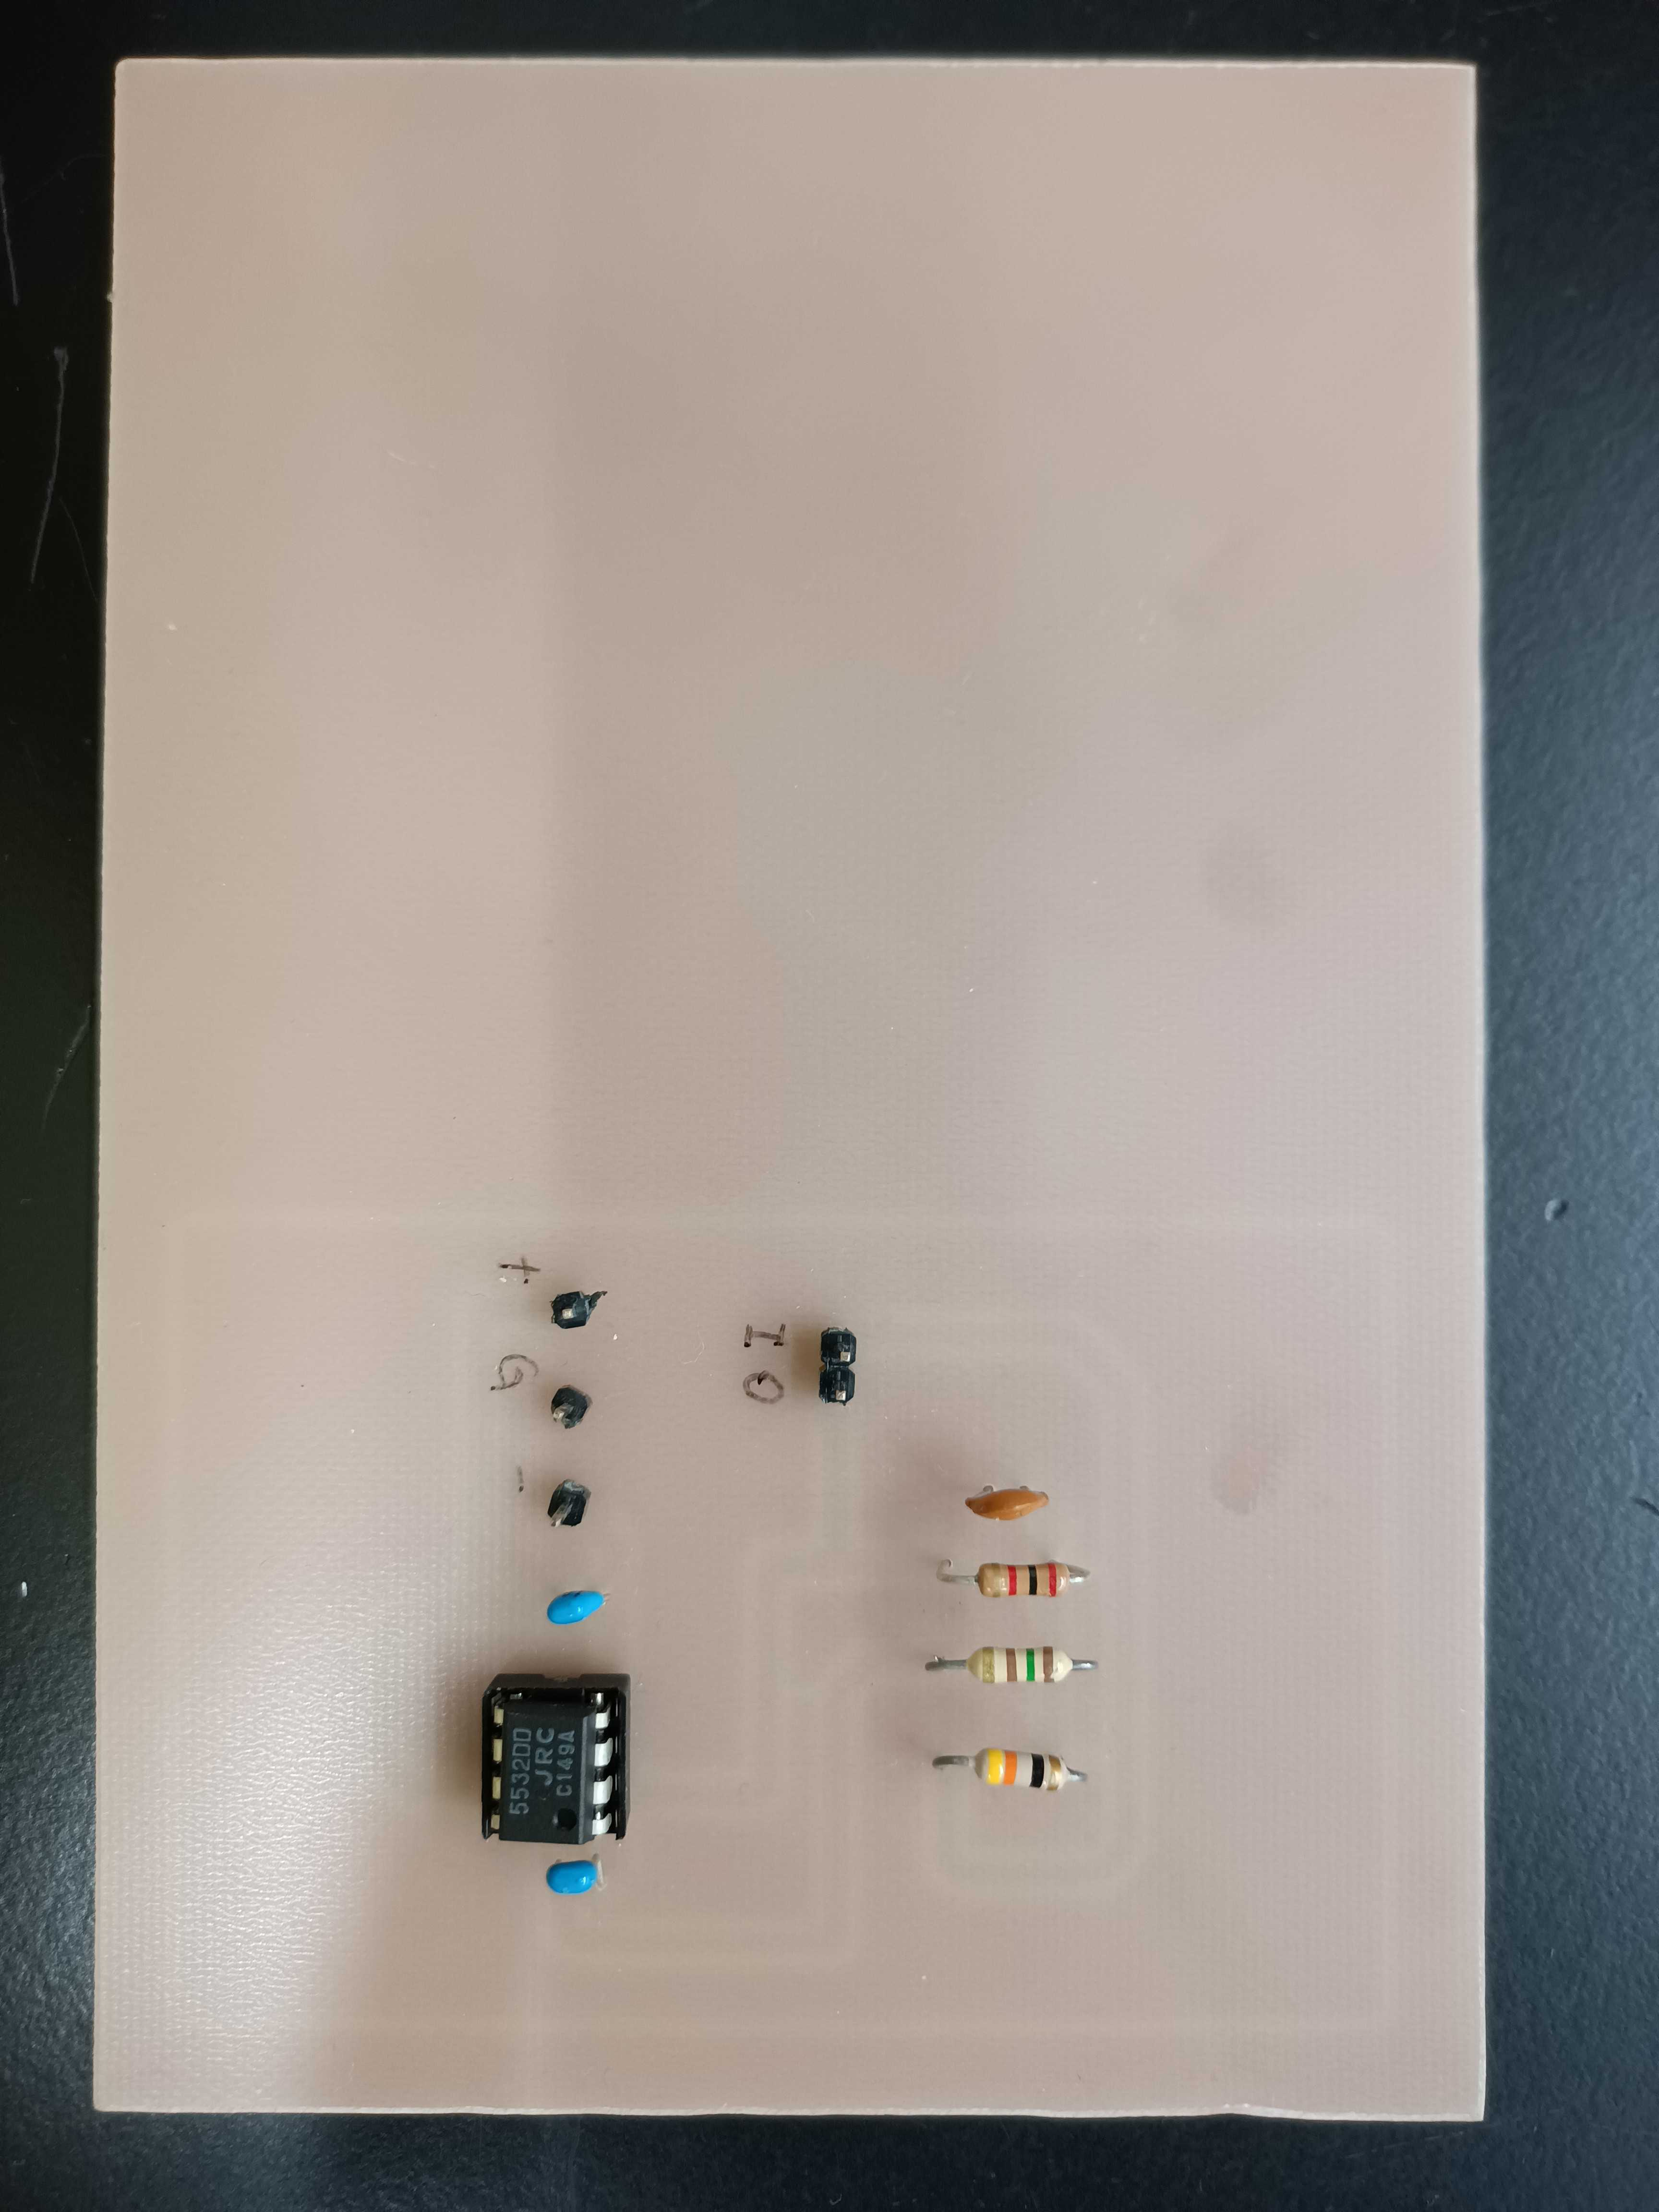
\includegraphics[width=8cm]{use/1.jpg}
		\caption{3号機アンテナの写真}
		\label{fig:s_7}
	\end{minipage}
\end{figure}

\subsection{役割分担}

役割分担で負担が偏ってしまった。

\end{document}
